%!TEX root = ../../main.tex

\chapter{Quantum computers and functional verification}

\section{Architecture, applications and challenges of quantum computers}

To understand the requirements a quantum computer poses to hardware design the main components of a quantum computer and the according concepts of quantum mechanics have to be understood. It is interesting to investigate what actually makes a quantum computer be superior to classical computers and which real-world applications this would impact. Finally the problem of quantum decoherence and its ramifications for building quantum computers should be examined.

\subsection{Qubits, superposition and fundamentals of quantum mechanics}

The main difference in between a classical and a quantum computer is that a quantum computer operates on quantum bits - so called \textit{"qubits"} - instead of bits. While a classical bit can only ever attain one of the values \texttt{0} and \texttt{1} a qubit can be in a \textit{superposition} of these two states. To portray this fundamental concept of quantum mechanics Erwin Schrödinger's crafted a popular thought experiment.

Schrödinger proposed to imagine leaving a cat inside a box for one hour together with a device containing a lethal poison. The device is constructed in such a way that it releases its mortal contents only on 50 percent of the attempts. Therefore upon opening the box one would always be equally probable to find the cat dead as one would to find her alive. \cite[see][p. 812]{Schr35} But what assertions could be made about the cat's condition before opening the box? Answering this questions incited heated discussions among physicists and to this point they haven't been able to find a common ground. One could maybe say she is both dead and alive and the only way to find out is by looking inside. Is it this "looking up"-process that actually determines the afterwards condition or has the cat been dead or alive all along? There are many different interpretations of quantum mechanics. For example the Copenhagen interpretation of quantum mechanics would argue that actually nothing can be said about the state of the cat before opening the box. Only predictions about probabilities can be made, until the act of measuring collapses the room of possibilities onto one determinate outcome - dead or alive.

This is the core of quantum mechanics - the concept of one thing being in a superposition of two states. The probability of either result to actually be achieved doesn't always have to be equal, but the main idea is that before measurement the cat is neither dead nor alive, the electron has neither up- nor down-spin and the qubit's state is neither \texttt{0} nor \texttt{1} - it's something in between.

\subsection{The essence of quantum supremacy}

\textit{Superposition} is why a quantum computer doesn't just work with two states per qubit. It works with a two-dimensional room of states for each qubit. But not just that, a quantum system with n qubits can be in a superposition of all $2^n$ possible solutions. Three qubits can collapse to the results \texttt{000}, \texttt{001}, \texttt{010} and so on. A superposition of these already covers an 8-dimensional room. This indicates that linear increase in amount of qubits leads to exponential growth in state space and already hints at the possible capabilities of quantum computers with large amounts of qubits. \cite[see][p. 308]{Rie98}

Quantum algorithms take advantage of that property via \textit{quantum parallelism} -  using its computational space to change a multitude of states at the same time. But every qubit measurement only ever leads to one of two solutions. Upon measurement qubits are equal to classical bits - they can't hold any more information. So one important part in quantum computing is to do operations while keeping the superposition of qubits alive which demands for completely different programming approaches. Possible operations are phase shifting certain inputs to increase the likelihood of them being measured or by extracting information all inputs share. The power of quantum computing lies in the fact that these operations change multiple inputs at once and possibly lead to a result way faster \cite[see][p. 317]{Rie98}.

An application that uses on of these approaches is \textit{Shor's algorithm}. It solves the popular problem of factorizing numbers and has been proven to do so in polynomial time. That makes it considerably more efficient than state of the art algorithms on classical computers that remain in exponential time complexity \cite[see][p. 251]{Kas06}. A big part of nowadays' internet transactions are secured by RSA encryption which is based mainly on the fact that large prime numbers are difficult to factorize. That means that if we succeed in building large enough quantum computers, Shor's algorithm would enable proprietors to eavesdrop in unknown dimensions. Advances in quantum computing therefore mandate a shift in transmission encryption. 

Quantum algorithms make use of another puzzling phenomenon of quantum mechanics: \textit{entanglement}. As the name already indicates two entangled quantum mechanical systems are deeply interdependent. Let two systems exist in a superpositional state such that the probability of each outcome depends on the outcome of the other. Lets imagine for example that two qubits will have equal probability of being measured as \texttt{00} and as \texttt{11} (the first number being the result of the first qubit, the second that of the second). That means there's a 50 percent chance for both options. If then the first qubit is measured and found out to be \texttt{0}, it's already known that the second qubit must be \texttt{0} too, because \texttt{01} as a a result has a probability of zero. So collapsing one quantum system immediately determines the state of the other - but not just that. It actually even leads to the other particle collapsing to the determined outcome. The most fascinating part is that apparently distance in between these systems doesn't matter. Two entangled particles can be light years apart - the "interaction" still takes place without visible or measurable communication. Even Albert Einstein was confused by this. He actually went as far as to claim that this disproves quantum mechanics altogether, because it stands in such convincing contradiction with his theory of general relativity which he used to show that there can be no communication taking place faster than the speed of light. It's called the \textit{EPR paradox} and it's been baffling minds for years \cite[see][p. 250]{Kas06}. As astonishing as it is, experiments have proven functionality of entanglement. At this moment there are quantum computers using it to their advantage. \textit{Grover's algorithm} employs these benefits in his search algorithm which works quadratically faster than the most efficient classical search algorithms \cite[cp.][p. 1]{Cha13}.

\subsection{The challenge of quantum decoherence}

As already mentioned a key component of quantum computing is being able to keep up the superpositional state of qubits. One measurement suffices to collapse a qubit to either \texttt{0} or \texttt{1}. But measurements don't always take place deliberately. Every interaction of a qubit with the outside world counts as a measurement. Losing superposition in such a manner is called \textit{quantum decoherence} and it's the major challenge to be overcome when building quantum computers. Coherence time is the time available for computation until a qubit collapses and its computational power is lost \cite[see][p. 251]{Kas06}.

There are several approaches to tackling this problem. Quantum \textit{error correction} is an algorithmic way of dealing with decoherence. It is similar to classical error correction, but made much more difficult by the fact that no qubit state can be copied and stored, because measurement leads to a loss of superposition. Error correcting algorithms use quantum parallelism and deliberate measure at the right time to outweigh environmental influences \cite[see][pp. 328f]{Rie98}. 

But there is also something to be done on the architectural side. Quantum computers can be build in a way that minimizes the risk of losing superposition. One way is to isolate the quantum chip as good as possible from the environment. This is why quantum computers still come in sizes that take up complete rooms and why we are very far from making quantum computing mobile. By isolation coherence time can be stretched out, but it also slows down operation time \cite[see][p. 39]{Meter06}. 

In order to maximize what can be achieved in the time available speed plays a vital role. Fast control operations are important not only because of decoherence-restricted time frames, but also because most quantum algorithms require a large amount of gates to compute the desired results. The solution of error-correcting algorithms indicated that fast measure is of equal priority as fast control \cite[see][pp. 33f]{Meter06}. This is why control units for quantum computers need to be designed using high-speed link-layer communication. Serial communication should be preferred to parallel communication, because of its advantages in speed \cite[cp.][p. 66]{Cai02}. Standard Ethernet doesn't suffice for these cases. Instead multi-gigabit transceivers should be chosen to guarantee usefulness of the architecture.

\begin{figure}[h]
  \centering
      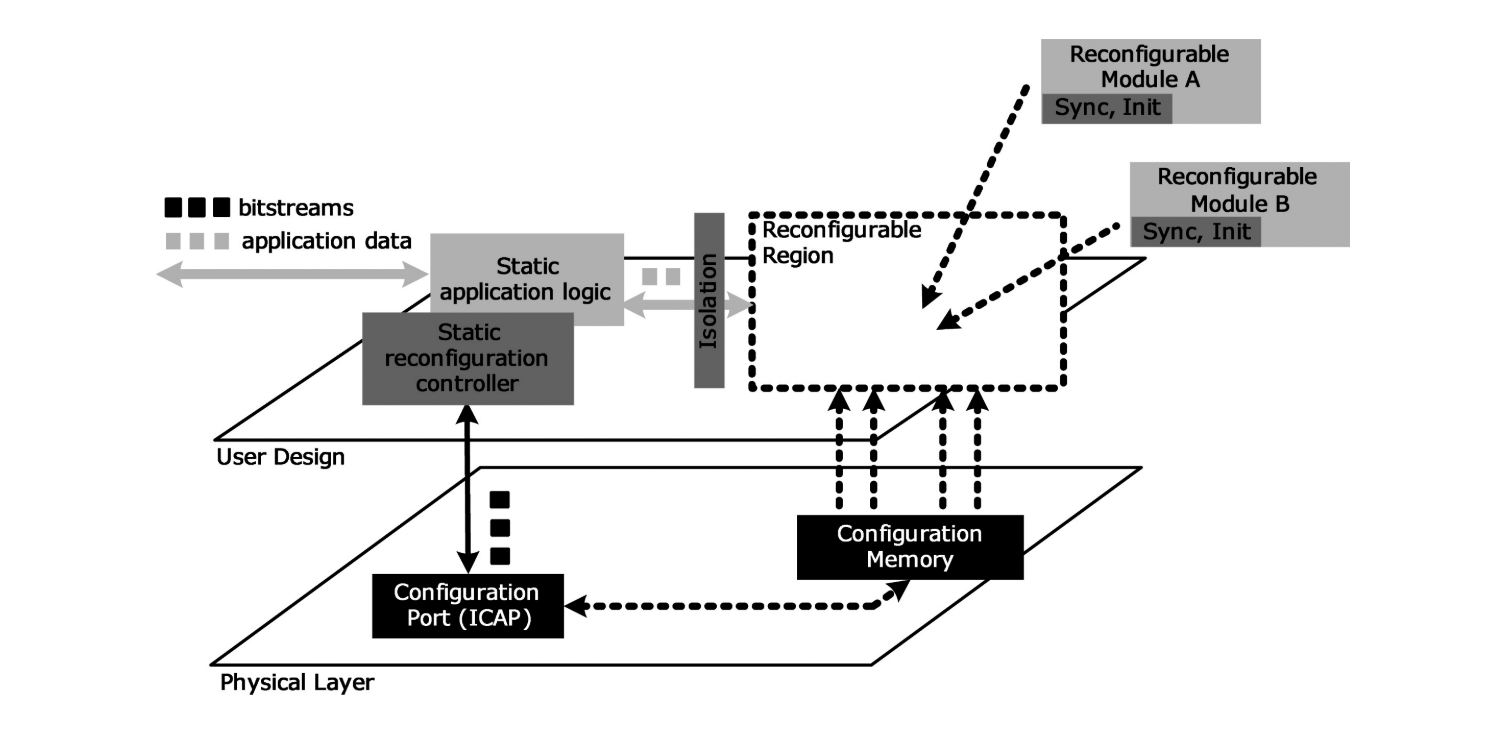
\includegraphics[width=0.7\textwidth]{drs}
  \caption[\acs{DPR} design] {Conceptual diagram of a \acs{DPR} design \cite[p. 97:3]{Gong14}}
  \label{fig:drs}
\end{figure}

Another factor in a research-driven domain as quantum computing is flexibility. This has implications that can be addressed using \acs{FPGA}s as a core integrated circuit in control units. Field-programmable gate arrays (\acs{FPGA}s) are reprogrammable chips. As can be seen in figure \ref{fig:drs} alongside several I/O pins an \acs{FPGA} consists of fixed parts that usually include RAM and a core processor on the one hand and programmable variable parts on the other hand. This enables dynamic partial reconfiguration (DPR) which makes the internal logic adjustable at runtime \cite[see][p. 97:1]{Gong14}. So in contrast to traditional \acs{IC}s an \acs{FPGA} doesn't have to be rebuild to change its logic blocks. It still offers the same functionality as a regular \acs{ASIC} (application-specific integrated circuit) that has to be reconstructed if changes are required after first design. This is especially interesting for emerging architectures but it comes with some downsides. An \acs{FPGA} generally takes up more space and operation time than an \acs{ASIC} \cite[see][p. 214]{Kuon07}. But an \acs{FPGA} can always be used to test and confirm the design and later be translated to an \acs{ASIC} to gain the advantages in performance. So in this project it made sense to use an \acs{FPGA} both because it was a fairly young project and because the context of quantum computing demands a certain flexiblity. The Xilinx Zynq-7000 \acs{SoC} - the \acs{IC} used on this project - is a system-on-a-chip that offers the programmability of an \acs{FPGA}.

The logic in an \acs{FPGA} is usually described using Hardware Description Languages (HDLs), e.g. VHDL or SystemVerilog. Hardware designers use these to express data flow typically on a degree of abstraction of the register-transfer level (RTL). So by HDL the designer defines the state of and operations on core registers. One doesn't have to write these hardware descriptions from scratch, but instead can refer to component-specific libraries or use the visual programming functionality of tools like the Vivado Design Suite.  Once the designer has committed his changes to the \acs{IC} the functional verification engineer comes into play.

\section{Functional verification and its tools}

Functional verification is responsible for making sure an architecture's functional requirements are being met. It is quite obvious that it plays quite a critical role in every design cycle. It is estimated that it costs up to 70 percent of a project's resources \cite[p. 286]{Fine03}. Functional verification is only one of several types of verification. There is also formal verification which tries to prove logically that a certain dysfunction can impossibly appear. In contrast functional verification strives to assure that errors are unlikely to happen by simulating the design logic as often as possible with a variety of test cases (behavioural simulation). This can be followed up by logic simulations that include the notion of timing to guarantee not only functional, but also timing requirements. To do so one uses \acs{HDL} simulators that emulate the behaviour of the developed design in a specific environment controling input and observing the output \cite[see][pp. 7ff]{Xi18}. There are many different approaches to follow, but one that tries to generalize a common way to go is the Universal Verification Methodology (UVM). 

\begin{figure}[h]
  \centering
      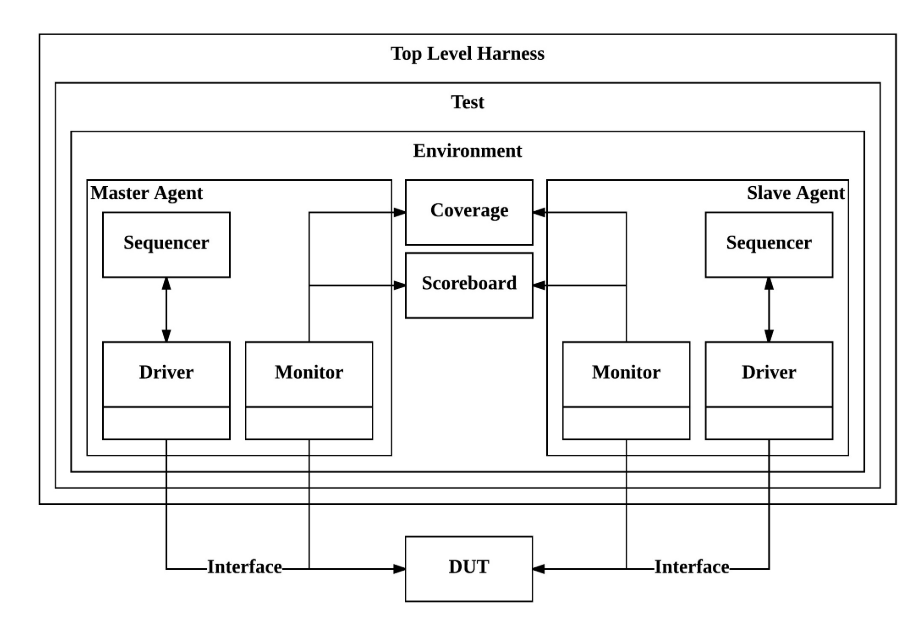
\includegraphics[width=0.7\textwidth]{uvm}
  \caption[\acs{UVM} testbench] {\acs{UVM} test bench architecture \cite{Pavi17}}
  \label{fig:uvm}
\end{figure}
\noindent
As seen in figure \ref{fig:uvm} \acs{UVM} test benches include all necessary components to stimulate, monitor and observe a device under test (DUT). The sequencer (also called generator) uses pre-defined \textit{constraints} to generate input that is then forwarded to the driver. The driver translates the given input into signals that can be processed by the \acs{DUT}. The monitor listens to the driver input, captures \acs{DUT} output and sends it to the scoreboard which possesses a previously defined \textit{reference model} that includes mappings for expected outputs. It compares monitored data and reports failures \cite[see][p. 2]{Pavi17}.
Capturing such a test in an \acs{HDL} representation allows for parsing and building of the according simulation models. Depending on the specified \acs{HDL} files, the simulation settings and the defined libraries a \textit{netlist} is generated which can be passed on to simulators. 

This project is working with two tools to complete these tasks which complicates and decelerates the overall build work flow necessary to simulate and verify new changes to the design. As aforementioned functional verification makes up a major bottleneck in every design cycle so clearly speed and automation in the simulation build are of particular interest. Before weighing possible technological solutions the present work flow needs to be investigated more in depth.